\documentclass{article}

\usepackage{amsmath}
\usepackage{graphicx}
\usepackage{float}

\title{M\o ller Event Selection\\and MC/Data Comparison\\in EngineeringRun2015}
\date{02-16-2017}
\author{Bradley Yale}

\begin{document}
	\pagenumbering{gobble}
	\maketitle
	\newpage
 	\pagenumbering{arabic}

\section{Introduction}

	\paragraph{}
	M\o ller scattering is a very useful process to be able to identify in HPS because of its well-known kinematics. This note describes how M\o ller electrons may be identified using cuts based on the elastic model to isolate them, followed by a cross section and mass resolution comparison between data and Monte Carlo simulations. The Monte Carlo shown will be separated into pure M\o llers, and M\o llers with the full beam background (wab-beam-tri) included.
	\paragraph{}
This document is based on 1.05 GeV run conditions, but the same principles apply at any beam energy. This analysis compares 'Pass 6' data with Monte Carlo that used the '3.10-20160813' HPS-jar. The detector geometry is 'HPS-EngRun2015-Nominal-v5-0-fieldmap'.

\section{The Elastic Model}

	\paragraph{}
	Elastic scattering in which an electron scatters from another electron follows a simple model, which relates its energy $E$ to the scattering angle $\theta$:

	\begin{equation}	\label{eq:ET}
  	E(\theta) = \frac{E_{beam}}{1+\frac{2E_{beam}}{m_e}\sin^2{\left(\theta/2\right)}}
	\end{equation}\newline

	In the case of the 2015 Engineering Run, $E_{beam} = \mbox{1.05 GeV}$. The curve which follows this model provides an excellent check of how closely a M\o ller candidate selected from a collection of vertexed electrons follows the expected scattering model. 
	To minimize accidentals, the primary M\o ller cuts imposed should involve both electrons selected from a vertexed pair rather than individual electrons, and it will also serve the interest of calibrating with their unique kinematics.

	\paragraph{}
	M\o llers in the HPS experiment should primarily come from a beam electron $\left(E=E_{beam}=\mbox{1.056 GeV}\right)$ that has been scattered from a target electron approximated to be initially at rest. In this case, the energies of the detected Moller pair should always add to the beam energy:

	 \begin{equation} \label{eq:EE}
  	E_2(E_1) = E_{beam} - E_1
	\end{equation}\newline 
	
	Enforcing the condition of elastic scattering, eq.(\ref{eq:ET}), and solving for $\theta_2$, a relationship between the two scattering angles of the M\o ller pair can be obtained as well:

	 \begin{equation} \label{eq:TT}
  	\theta_2(\theta_1) = 2\sin^{-1}{\left(\frac{m_e}{2E_{beam}}\csc{\left(\theta_1/2\right)}\right)}
	\end{equation}\newline 

	Together, eqs.(\ref{eq:ET}), (\ref{eq:EE}), and (\ref{eq:TT}) can be used to demonstrate how closely selected electrons obey the elastic model, before and after the distributions get smeared by HPS. Agreement with this model from pre-SLIC Monte Carlo M\o llers is near-perfect, as seen in figures \ref{fig:stdEE}, \ref{fig:stdTT}, and \ref{fig:stdET}.
	
	\begin{figure}[H]
  	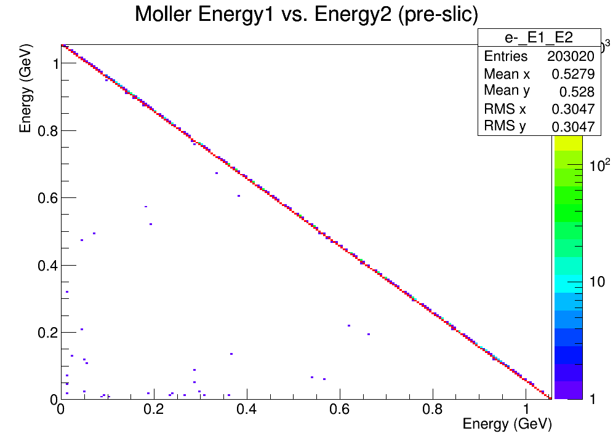
\includegraphics[width=\linewidth]{old/stdEE.png}
  	\caption{$E_1$ vs. $E_2$ of M\o ller stdhep events just after the target (Curve: eq.\ref{eq:EE})}
  	\label{fig:stdEE}
	\end{figure}
	
	\begin{figure}[H]
  	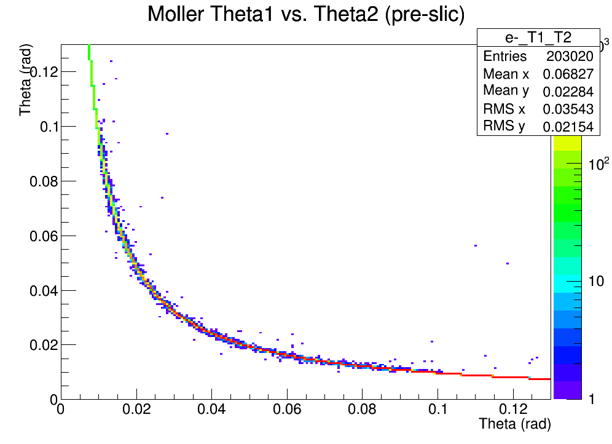
\includegraphics[width=\linewidth]{old/stdTT.png}
  	\caption{$\theta_1$ vs. $\theta_2$ of M\o ller stdhep events just after the target (Curve: eq. \ref{eq:TT})}
  	\label{fig:stdTT}
	\end{figure}
	
	\begin{figure}[H]
  	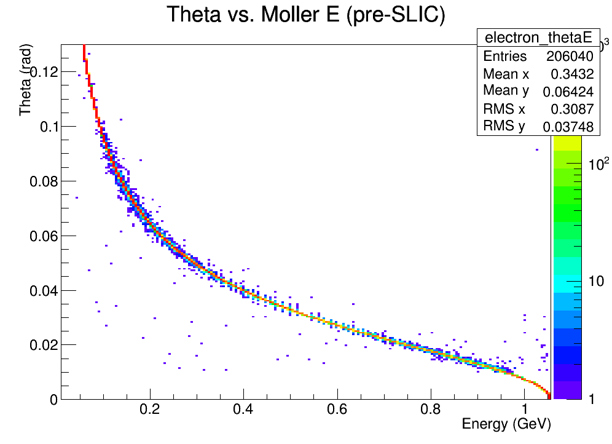
\includegraphics[width=\linewidth]{old/stdET.png}
  	\caption{Energy vs. $\theta$ of M\o ller stdhep events just after the target. The low-energy tail is due to multiple scattering within the target (Curve: eq. \ref{eq:ET})}
  	\label{fig:stdET}
	\end{figure}

	From the tails of these distributions, and considering that multiple scattering within the target creates (identifiable) events with photons and positrons, this indicates that up to 95\% of events using this generator can be confidently identified as Moller events after reconstruction. It is also important to note that all scattering angles used in this study are rotated by $-30.5$ mrad in $\theta_x$, to undo the beam offset that the simulations also take into account. Any analysis cut which assumes a scattering angle between the momentum at the target and $(0,0,\vec{k})$ must apply this correction as well.

\section{Normalization}
\paragraph{}
The following 1-D distributions  are normalized by 1/Luminosity such that the histograms will integrate to give the respective M\o ller cross sections in units of millibarns. The Monte Carlo luminosity is obtained from the time structure of the simulated beam and the HPS target parameters:

\begin{equation} \label{eq:MCLumin}
	\begin{split}
  	Lumin_{MC} =(\#\mbox{ files})*(\mbox{74 scatterers/atom})*(\#\mbox{ bunches})*(\mbox{625 electrons/bunch})
  	\\*(4.062*10^{-4}\mbox{ atoms/cm/barn})*(6.306*10^{-2}\mbox{ cm})
  	\end{split}
	\end{equation}

The 625 electrons/bunch comes from the 2ns/bunch time structure representing a current of 50nA for the 2015 running. The number of electron beam bunches incident on the target for pure Mollers is 2 million; for 'wab-beam-tri' (WBT), the Monte Carlo which represents Mollers with the full beam background included, 500k incident electron bunches are sent to the target. These numbers should be kept in mind when normalizing, and adjusted accordingly if ever changed at generation.

\paragraph{}
Distributions produced from reconstructed data must additionally take the prescale factor into account, since for Monte Carlo readout, $prescale_{MC}=2^0=1$ (same as for the pair1 trigger in data). The trigger-dependent corrected luminosity for the full Run 5772 data set from 2015 is then:

\begin{equation} \label{eq:DataLumin}
	Lumin_{Data} =2^{prescale}*42.36560598*10^{9}\mbox{ }barns^{-1}
	\end{equation}\newline

The luminosity used for data is already corrected for inefficiencies such as SVT bias and livetime. Since the 2015 run did not have a trigger designed specifically for Mollers, the singles1 trigger was used for this study, which had a prescale factor of  '11'. Therefore, the singles1 data luminosity differs in normalization from MC by an overall factor of $2^{11}=2048$, excluding any additional unknown MC/Data discrepancies.
\paragraph{}
The normalized energy distributions of the generated M\o llers before the target ($>5mrad$,$>10 MeV$ cuts) follows the M\o ller cross section in literature (Messel and Crawford), as seen in figure \ref{fig:XS}. %Explicitly, this differential M\o ller cross section is

%\begin{equation} \label{eq:MollerXS}
%	\begin{split}
  %	\frac{d\sigma}{dE} =
  %	\end{split}
	%\end{equation}

\begin{figure}[H]
  	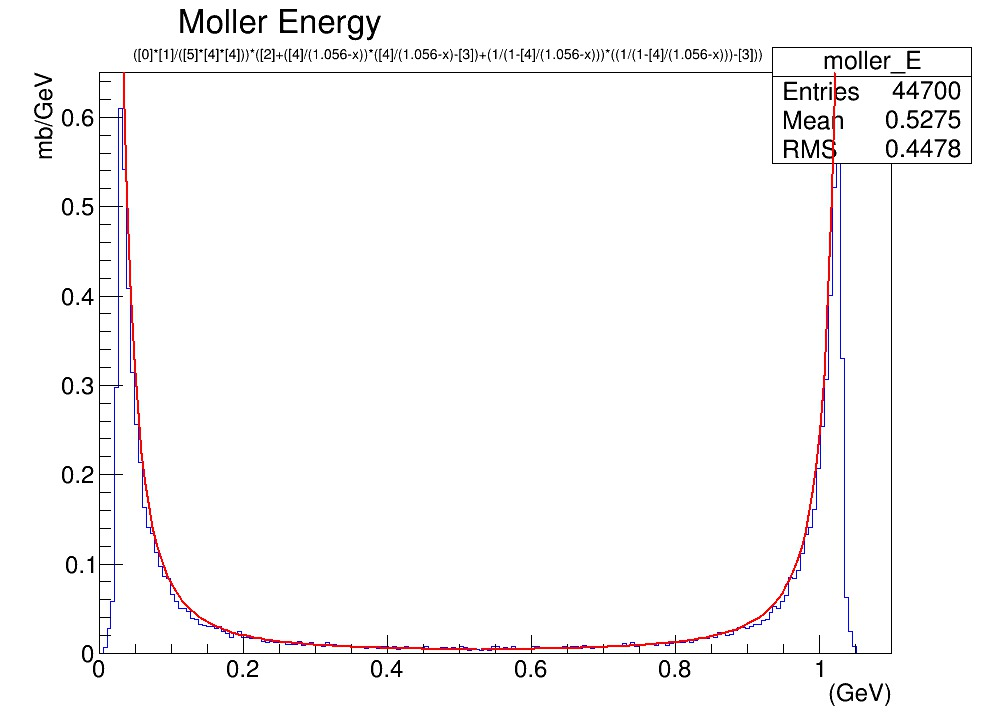
\includegraphics[width=\linewidth]{MollerPlots/MollerXS.jpg}
  	\caption{Energy distribution of Pure M\o ller events just after the target, with cross section model overlain.}
  	\label{fig:XS}
	\end{figure}

\begin{figure}[H]
  	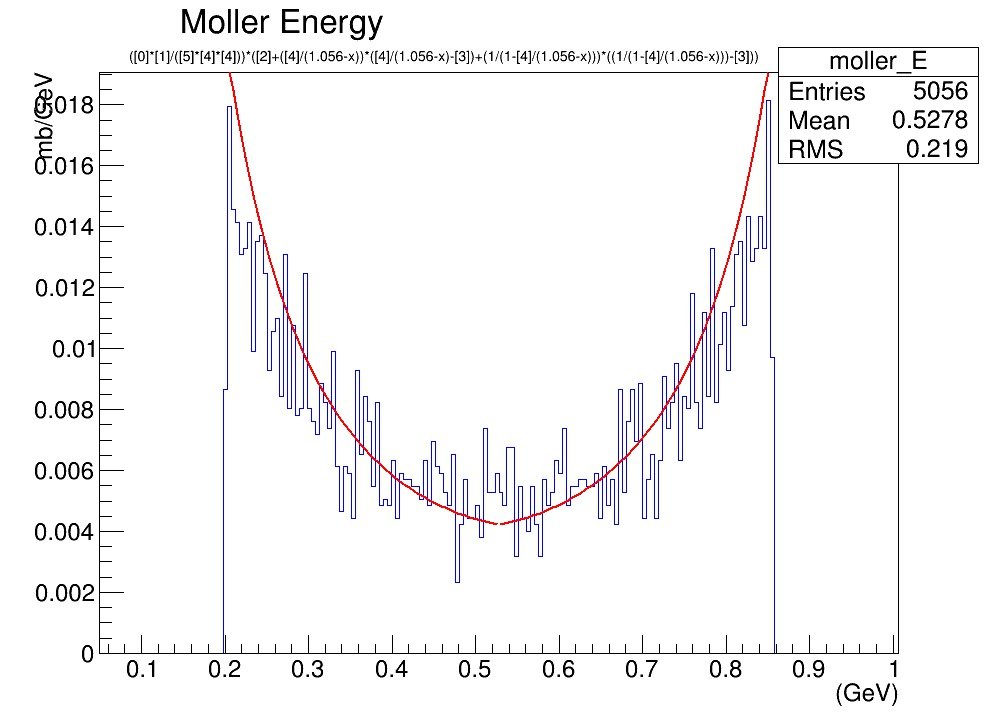
\includegraphics[width=\linewidth]{MollerPlots/MollerXS_acceptance.jpg}
  	\caption{Energy distribution of Pure M\o ller events just after the target, with cross section model overlain, within the range [0.2, 0.8 GeV]. Integrated cross section for histogram (model): 5.340 mb (5.498 mb).}
  	\label{fig:XSAcceptance}
	\end{figure}

The cross sections are calculated in figure \ref{fig:XSAcceptance} from the range 0.2 to 0.8 GeV to match the 1.056 GeV energy acceptance of HPS after full reconstruction, seen in figure \ref{fig:energyRecon}.

\begin{figure}[H]
  	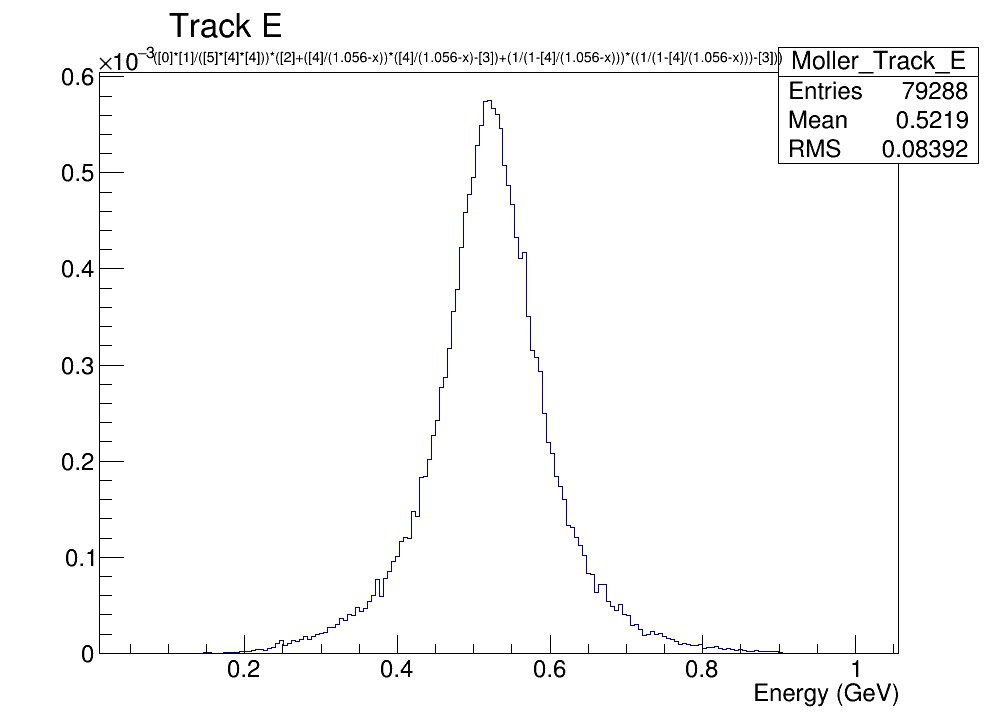
\includegraphics[width=\linewidth]{MollerPlots/MollerXS_Recon.jpg}
  	\caption{Energy distribution of Pure M\o ller Monte Carlo events after HPS reconstruction.}
  	\label{fig:energyRecon}
	\end{figure}

M\o ller selection cuts were determined to efficiently extract M\o ller electrons from this energy range.

	\section{M\o ller Selection Cuts}
	\paragraph{}
	'MollerCandidates' is a collection of HpsParticles available in the standard HPS recon output since 'Pass 2', and includes vertexed pairs of electrons using the same vertexing procedure as for usual electron-positron pairs, except that the tracks are constrained to both have a negative charge, and hits must be on opposite volumes of the ECal $\left(\tan{\left(\lambda_1\right)}*\tan{\left(\lambda_2\right)}<0\right)$. The following analysis will feature target-constrained (and later beamspot constrained) MollerCandidates containing GBL tracks only (TrackType$>$32), and the condition that each event must contain $>$1 track and $>$1 one cluster. If one of the vertexed electrons fails a particular cut, then the entire event is discarded, since the accuracy of the pair-dependent selection relies on both of these electrons being identified correctly. No $\chi^{2}$ cuts are made, since even loose ones reject too many events while having no appreciable effect on the M\o ller distribution shapes.

\paragraph{}
A set of M\o ller selection cuts was found (eqs. \ref{eq:CoinCutMeow} - \ref{eq:TSumCutMeow}), which recovers the relative cross sections from the normalized electron distributions after reconstruction, within the present efficiency of $20\%$ for a vertexed $e^+e^-$ pair:

           \begin{equation} \label{eq:CoinCutMeow}
  	-1.7 ns < (Cluster Hit Time_{1} - Cluster Hit Time_{2}) < 1.7 ns
	\end{equation}
	
	\begin{equation} \label{eq:PCut}
  	 Track Momentum<0.85 GeV
	\end{equation}
	
          \begin{equation} \label{eq:PSumCut}
  	Momentum_1 + Momentum_2<1.2 GeV
	\end{equation}

          \begin{equation} \label{eq:MatchingCut}
	\begin{split}
  	-15mm < [Cluster Seed Position_{x} - Cluster Track Position_{x}] < 15mm
  	\\-20mm < [Cluster Seed Position_{y} - Cluster Track Position_{y}] < 20mm
	\end{split}
	\end{equation}

	\begin{equation} \label{eq:TSumCutMeow}
  	50 mrad < \theta_1+ \theta_2 < 80 mrad
	\end{equation}\newline
	
	These cuts are shown in the relevant distributions, figures \ref{fig:CoinCutPlot} - \ref{fig:TSumCutPlot}.

	\begin{figure}[H]
  	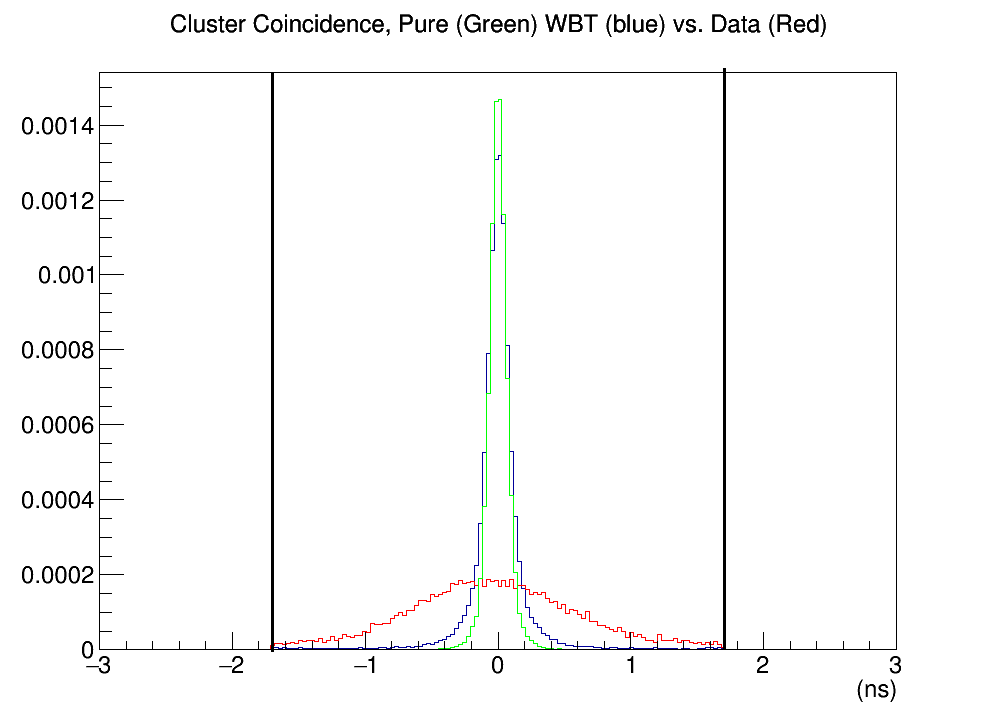
\includegraphics[width=\linewidth]{MollerPlots/ALL_Coincidence}
  	\caption{Cluster coincidence cut. Setting the range to $\pm1.7$ ns fully eliminates the sharp WBT background peaks at $\pm2$ ns and beyond.}
  	\label{fig:CoinCutPlot}
	\end{figure}

\begin{figure}[H]
  	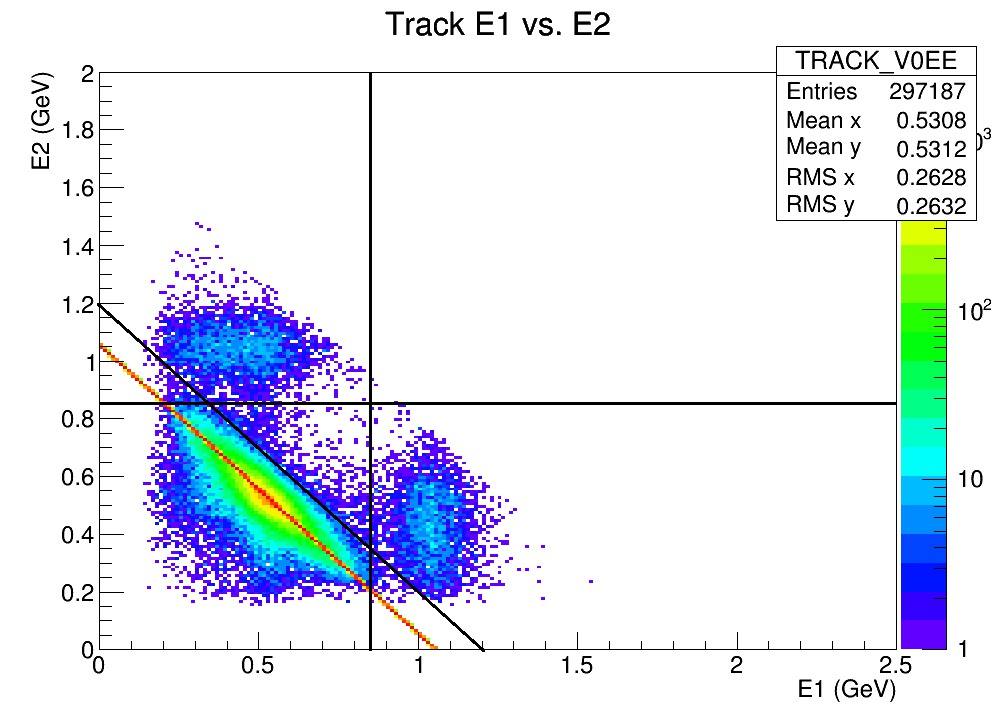
\includegraphics[width=\linewidth]{MollerPlots/DATA_TrackEE_cut}
  	\caption{Momentum and Momentum Sum cuts in Momentum1-Momentum2 space. The extraneous FEE peaks can be clearly seen at 1.056 GeV.}
  	\label{fig:MomCutsEE}
	\end{figure}

\begin{figure}[H]
  	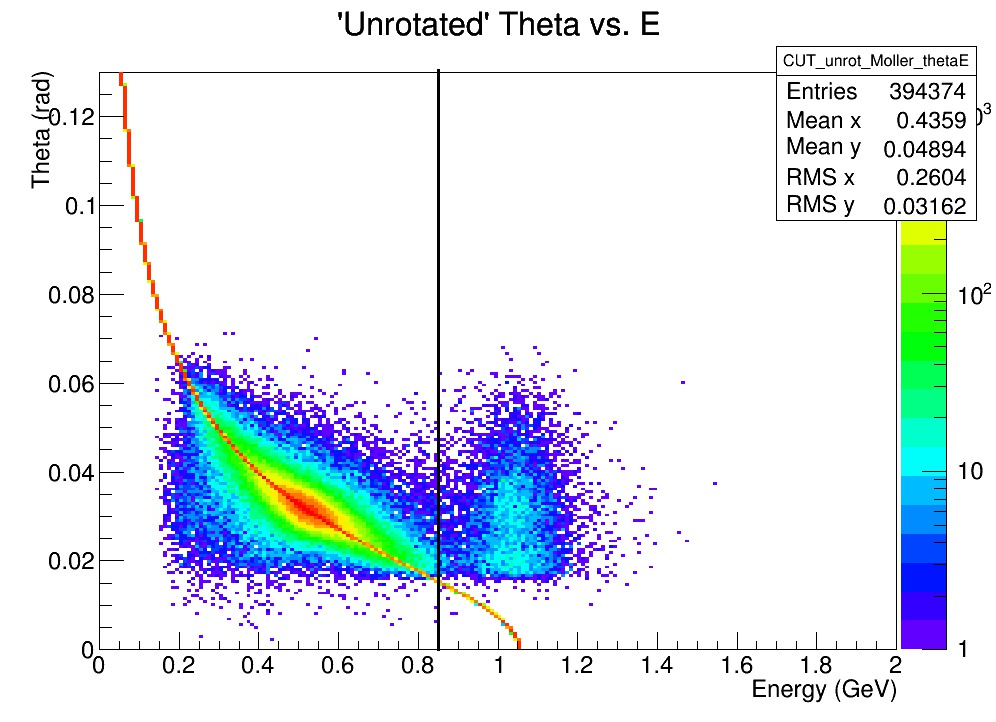
\includegraphics[width=\linewidth]{MollerPlots/CUT_Unrotmoller_ThetaE_cut}
  	\caption{Momentum cut in Theta-Momentum space. The extraneous FEE peak can be clearly seen at 1.056 GeV.}
  	\label{fig:MomCutsET}
	\end{figure}

\begin{figure}[H]
  	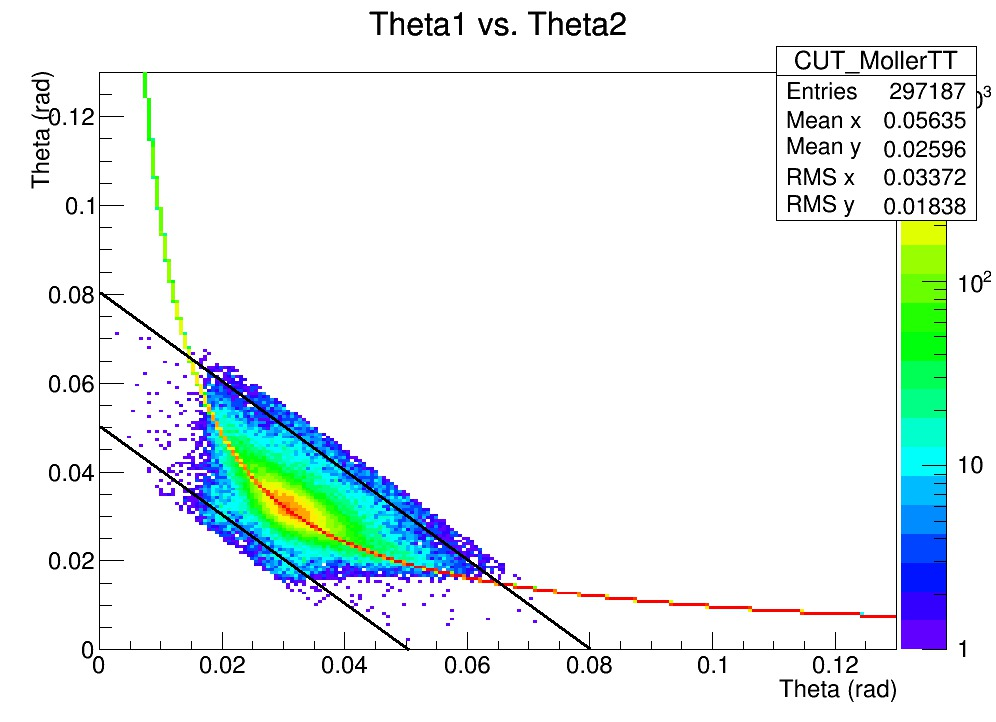
\includegraphics[width=\linewidth]{MollerPlots/CUT_PlotTT_cut}
  	\caption{Theta Sum cut. This cut is useful for selecting the now-triangular signal region in Theta1-Theta2 space after HPS recon.}
  	\label{fig:TSumCutPlot}
	\end{figure}

The effect on the invariant mass distribution from applying these cuts can be seen in figures \ref{fig:massUncut1} and \ref{fig:massCut1}.

\begin{figure}[H]
  	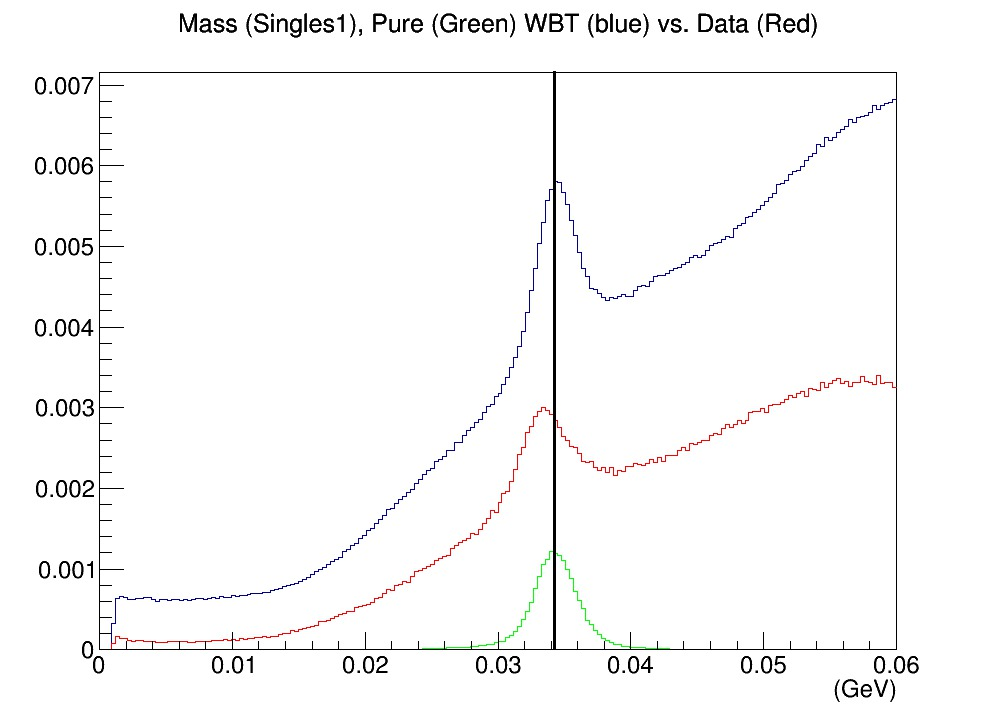
\includegraphics[width=\linewidth]{MollerPlots/ALL_massSingles1_shift}
  	\caption{Invariant mass distributions of \textit{all} MollerCandidates which passed the singles1 trigger in Pure MC (green), WBT (blue), and Data (red). Note the leftward shift in the Data peak.}
  	\label{fig:massUncut1}
	\end{figure}

\begin{figure}[H]
  	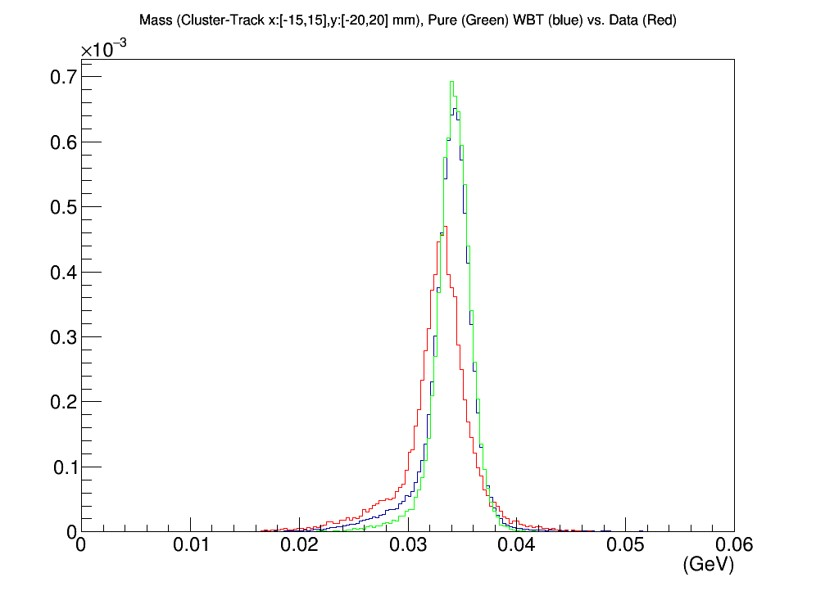
\includegraphics[width=\linewidth]{MollerPlots/massWithMatching}
  	\caption{Invariant mass distributions of the MollerCandidates which pass the selection cuts. \newline\newline Fit mass peaks (Gaussian+Exp):\newline WBT peak: Mean=34.34 MeV,  $\sigma_m/m = 3.8\%\newline$ Data peak: Mean=33.25 MeV, $\sigma_m/m = 4.7\%$.\newline\newline There is a $\sim1$ MeV shift between the MC and Data peaks, but this is eliminated by including a beamspot constraint.}
  	\label{fig:massCut1}
	\end{figure}

\begin{figure}[H]
  	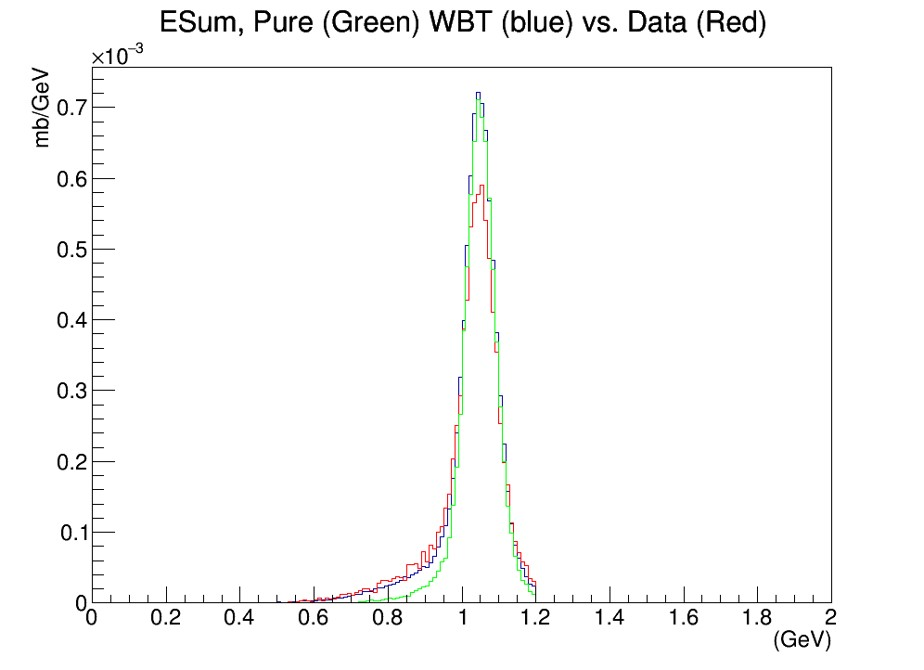
\includegraphics[width=\linewidth]{MollerPlots/TrackESum}
  	\caption{Track momentum sum of the MollerCandidates which pass the selection cuts. The two MC with and without background match in the signal region, while the WBT tail matches Data. Signal $\sigma_P/P = 3\%$}
  	\label{fig:CutMomSum}
	\end{figure}

Fitting the distributions after these cuts with a Gaussian+Exponential, the MC/Data cross sections differ by 18\%, which is within the $\sim 20\%$ discrepancy seen in recent trident studies. The worrisome feature of this cut mass spectrum is a systematic shift in the Data peak by $\sim$ 1 MeV, independent of trigger, as seen in the pair1 plot (\ref{fig:massCut1Pairs}).

\begin{figure}[H]
  	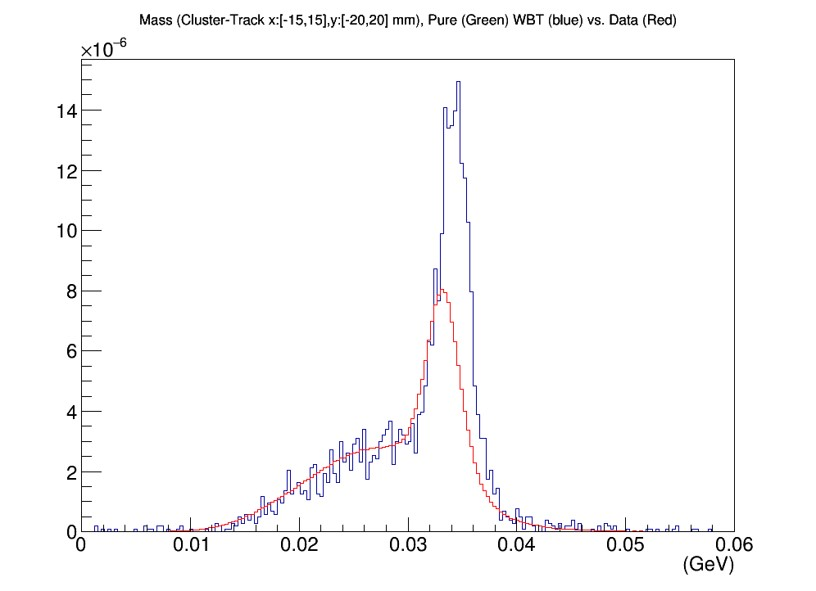
\includegraphics[width=\linewidth]{MollerPlots/massWithMatchingPairs}
  	\caption{Invariant mass distributions of the MollerCandidates which pass the selection cuts, with pairs1 trigger. The shift in the mass peak is still present, despite agreement in the tail/background regions. Since practically all M\o llers fail the pair1 coplanarity cut ($<$40 deg), the Pure M\o ller pair1 yield was negligible with current statistics, so not shown.}
  	\label{fig:massCut1Pairs}
	\end{figure}

While the source of this shift is unknown, it is able to be corrected by tightening the target constraint into a beamspot constraint. The resulting mass distribution is figure \ref{fig:massCut2}.

\begin{figure}[H]
  	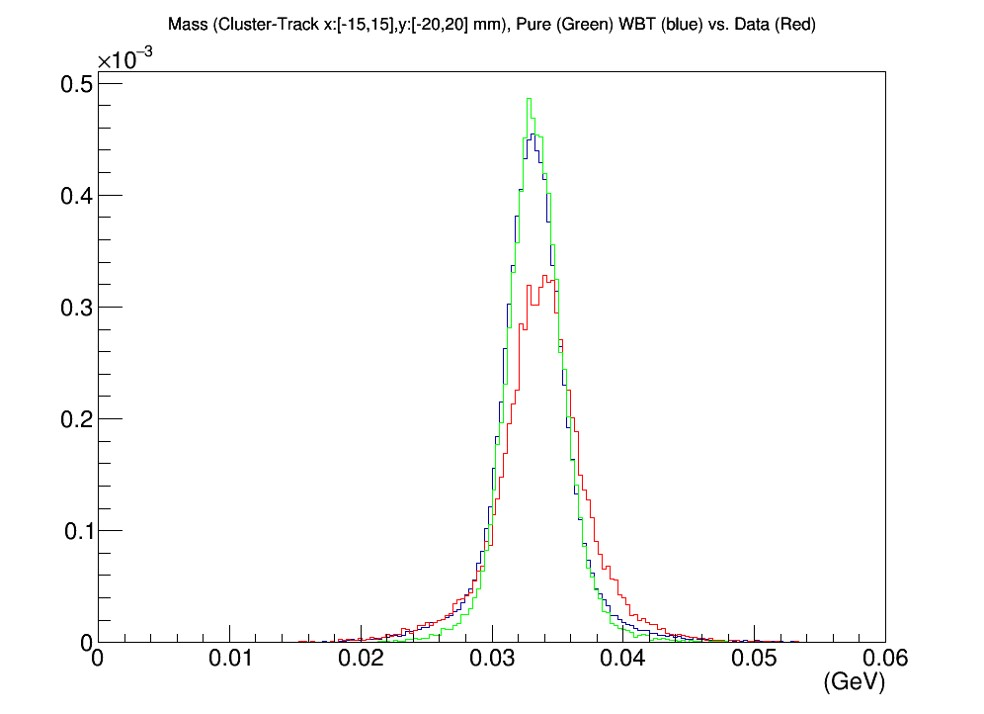
\includegraphics[width=\linewidth]{MollerPlots/massWithBSC}
  	\caption{Invariant mass distributions of the singles1 MollerCandidates which pass the selection cuts, as well as the constraint that the vertex falls within the beamspot. Beamspot Gaussian width: (130,50 um).\newline\newline Fit mass peaks (Gaussian+Exp): \newline MC peak: Mean=33.33 MeV,  $\sigma_m/m = 5.5\%$\newline Data peak: Mean=33.84 MeV, $\sigma_m/m = 6.8\%$}
  	\label{fig:massCut2}
	\end{figure}

\begin{equation} \label{eq:MollerMass}
  	\mbox{M\o ller Invariant Mass} = \sqrt{2m_e^2 + 2E_{beam}m_e} = 32.86 MeV
	\end{equation}\newline

Adding the beamspot constraint shifts the mass peaks closer to the calculated value of 32.86 MeV (eq. \ref{eq:MollerMass}), bringing the difference between MC and Data within 0.6 MeV (2.5 $\sigma$). This comes with the cost of widening the resolutions of both MC and Data by $\sim 2\%$, but they are still between the established energy resolution of $\sim 4.5\%$, and momentum resolution of $\sim 6.5 \%$.

\paragraph{}
While these cuts already demonstrate good MC/Data agreement, further improvements can be made, particularly with a low momentum sum cut

 \begin{equation} \label{eq:PSumCut}
  	Momentum_1 + Momentum_2>0.9 GeV
	\end{equation}

Adding this cut marginally  improves both the mass peak agreement between MC and Data, as well as the cross section.

\begin{figure}[H]
  	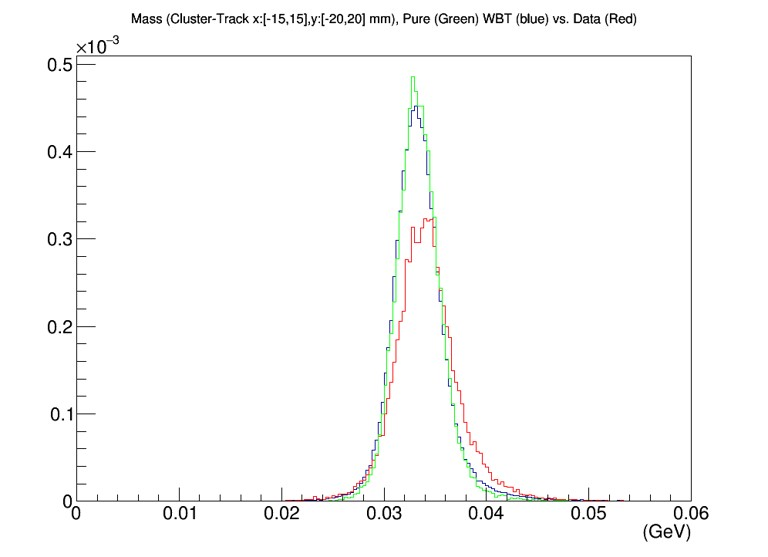
\includegraphics[width=\linewidth]{MollerPlots/massTightESum}
  	\caption{Invariant mass distributions of the singles1 MollerCandidates which pass the selection cuts, as well as the beamspot constraint and low PSum cut.\newline \newline Fit mass peaks (Gaussian+Exp): \newline Pure: Mean=33.29 MeV,  $\sigma$=2.001 MeV $(6.0\%)$\newline WBT: Mean=33.23 MeV, $\sigma$=2.025 MeV $(6.1\%)$\newline Data: Mean=33.81 MeV, $\sigma$=2.541 MeV $(7.5\%)$.}
  	\label{fig:massTightPSum}
	\end{figure}

Fitting fig. \ref{fig:massTightPSum} with a Gaussian+Exponential, this set of selection cuts brings the mean mass peak agreement between MC and Data to within 0.58 MeV, but the mass resolutions increase by nearly $+0.5\%$ with respect to figure \ref{fig:massCut2}. This resolution is likely more accurate however, as $\sim2$ MeV has been on the lower end of the sigmas seen in other studies; anything smaller than that, especially if it comes with an unexpected shift in the mean, is more likely to be artificial.

\paragraph{}
Integrating the background-subtracted Gaussian signals, the accepted cross sections differ by:\newline
\newline
1-WBT/PURE=$2.4\%$\newline
1-DATA/PURE=$15.3\%$\newline
1-DATA/WBT=$13.2\%$\newline

The Data/MC difference for M\o llers selected with these cuts is therefore at least $5\%$ better than the $\sim 20\%$ difference seen in tridents, with only a $2.4\%$ reduction in the MC signal with respect to pure M\o llers.

\section{Track/Cluster Energy Discrepancy}
\paragraph{}
Even with a good M\o ller selection, there is still a "leakage" effect for electrons which hit the edge crystals of the ECal, where the calibrations are not as accurate as for the fiducial region, and some of the hits in the cluster spill over into the opposite ECal volume. This causes the cluster energies to drift below the energy that the unaltered tracks suggest that the M\o ller should have.

\begin{figure}[H]
  	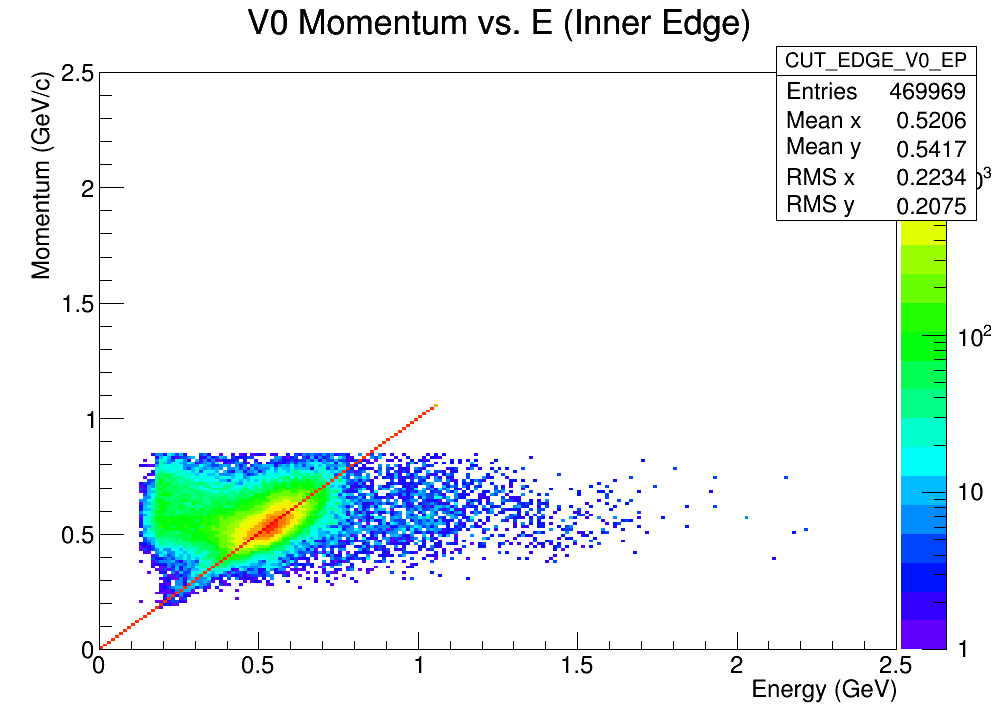
\includegraphics[width=\linewidth]{MollerPlots/EDGE_EP_bsc}
  	\caption{Track vs. Cluster Energy for beamspot constrained M\o llers passing the selection cuts (WBT shown), and with seeds on the edge ECal crystals. Many electron tracks in the M\o ller peak region ($E_{beam}/2$) are attached to clusters with 25-70\% lower energy than the tracks suggest.}
  	\label{fig:EPEdge}
	\end{figure}

\begin{figure}[H]
  	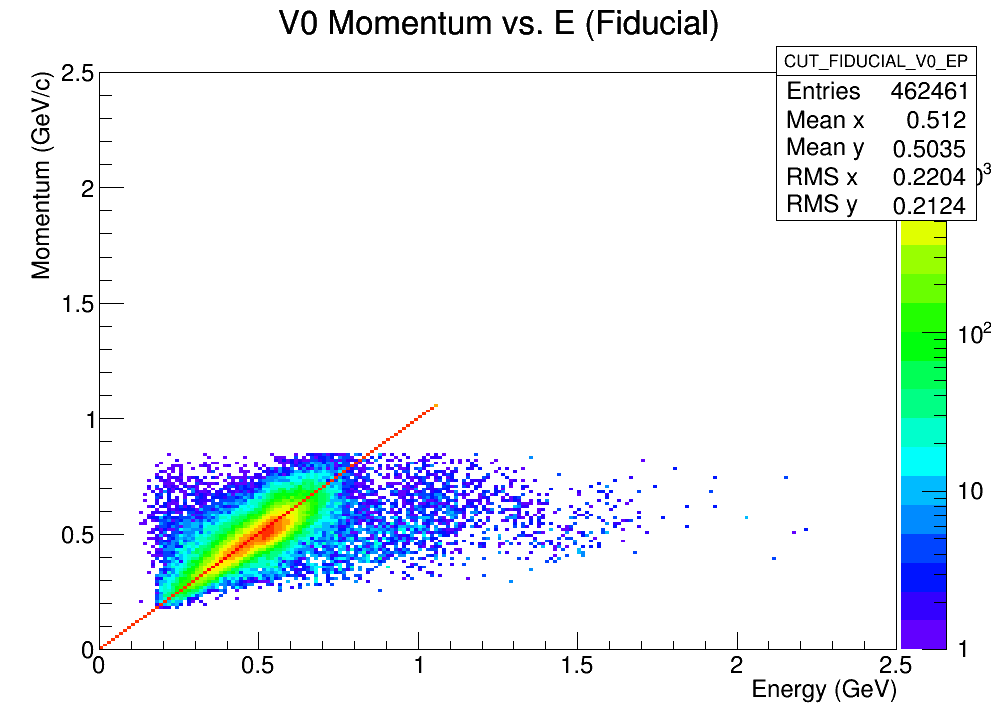
\includegraphics[width=\linewidth]{MollerPlots/FIDUCIAL_EP_bsc}
  	\caption{Track vs. Cluster Energy for Beamspot constrained M\o llers passing the selection cuts (WBT shown), and with seeds in the fiducial region of the ECal (not adjacent to a gap). The cluster/track energy agreement is far better in the fiducial region.}
  	\label{fig:EPFiducial}
	\end{figure}

In an attempt to select M\o llers with better agreement by adding a \textit{cluster} energy sum cut to match the momentum sum cut in the existing list ($0.9<Sum<1.2 GeV$), the track vs. cluster energy agreement is greatly improved over the entire ECal:

\begin{figure}[H]
  	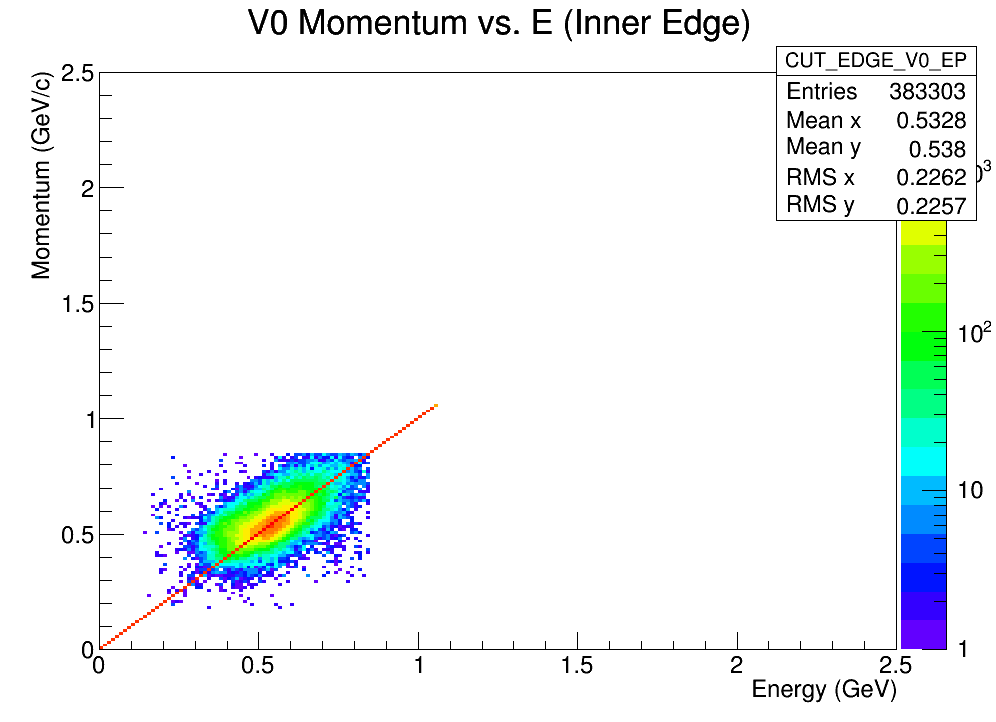
\includegraphics[width=\linewidth]{MollerPlots/EDGE_EP_tightPSum}
  	\caption{Track vs. Cluster Energy for beamspot constrained M\o llers passing the selection cuts (WBT shown), and with seeds on the edge ECal crystals. $0.9 GeV<Cluster ESum<1.2GeV$. The disagreement at low cluster energy is no longer present.}
  	\label{fig:EPEdge2}
	\end{figure}

\begin{figure}[H]
  	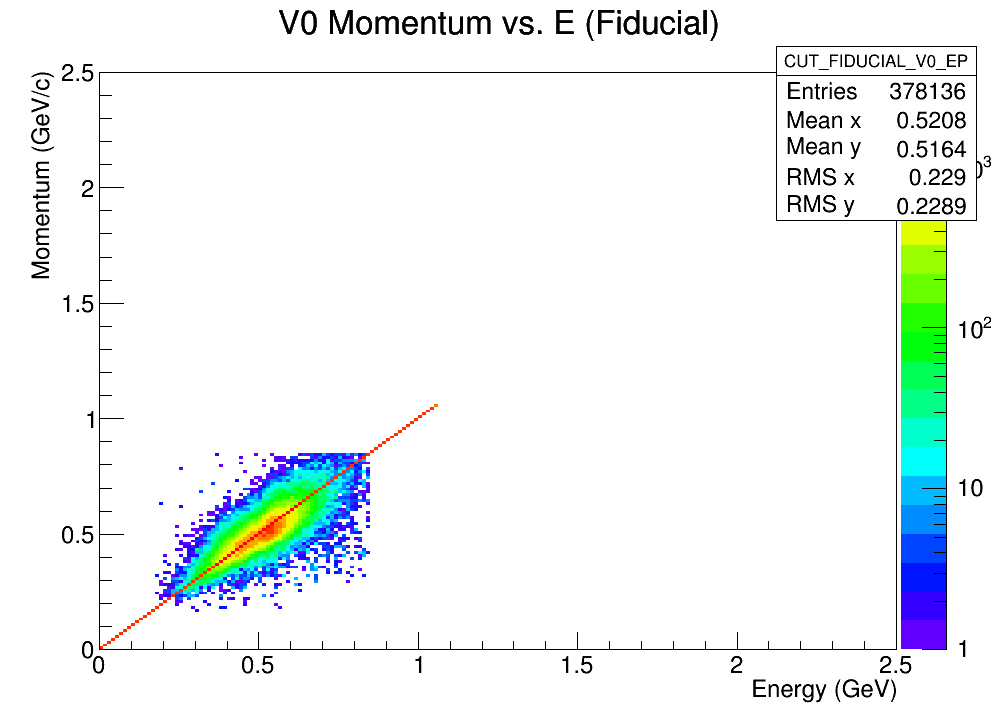
\includegraphics[width=\linewidth]{MollerPlots/FIDUCIAL_EP_tightPSum}
  	\caption{Track vs. Cluster Energy for beamspot constrained M\o llers passing the selection cuts, and with seeds in the fiducial region of the ECal (not adjacent to a gap). $0.9 GeV<Cluster ESum<1.2GeV$.}
  	\label{fig:EPFiducial2}
	\end{figure}

However, while this cluster ESum cut is an ad hoc way of selecting well-calibrated M\o llers, it also destroys the near-perfect agreement between WBT and Pure M\o ller MC. Checking the fitted cross sections, they now differ by:
\newline\newline
1-WBT/PURE=$18.6\%$\newline
1-DATA/PURE=$27.3\%$\newline
1-DATA/WBT=$10.67\%$\newline

While the WBT/Data difference is reduced to nearly $10\%$ by adding an additional cut on cluster energy sum, now both WBT and Data have lost an additional $12-16\%$ of their signal relative to the Pure M\o ller sample. This cut should then likely not be applied if the maximum number of accepted M\o llers is desired, but could be useful for studying the region very close to the M\o ller signal. The corresponding mass resolutions are (likely artificially) cut in half.
\newline \newline Fit mass peaks (Gaussian+Exp): \newline Pure: Mean=34.3 MeV,  $\sigma$=1.319 MeV\newline WBT: Mean=34.27 MeV, $\sigma$=1.263 MeV\newline Data: Mean=33.20 MeV, $\sigma$=1.557 MeV

\section{Summary}
\paragraph{}
Using the selection cuts from this note on beamspot-constrained MollerCandidates, GBL tracks only, with cuts from eqs. \ref{eq:CoinCutMeow} - \ref{eq:TSumCutMeow}, as well as a low momentum sum cut (\ref{eq:PSumCut}), M\o ller electrons can be reliably extracted from 1.056 GeV Monte Carlo and Data with a difference in MC/Data cross sections of $\sim 15\%$. This MC/Data difference is within the $20\%$ difference ($10\%$ for each track) seen in tridents. 
\paragraph{}
The mass resolutions with this selection criteria is 2 MeV $(6\%)$ for MC, and 2.5 MeV $(7.5\%)$ for data, within the momentum resolution of HPS. Since these cuts only reduce the M\o ller signal from the full background Monte Carlo with respect to the pure M\o llers by $2.4\%$ , it suggests that this is a set of reasonable M\o ller selection cuts, and most of the discrepancy between MC and Data is likely to come from elsewhere, such as radiative corrections or resolution differences between MC and Data. The background-subtracted integrated M\o ller cross section in Data is lower with respect to MC by $13\%$, and the M\o ller mass resolution is greater by $1.5\%$ with these selection cuts.
\paragraph{}
If an additional cut is desired to clean up the momentum vs. cluster energy discrepancy on the edge crystals while avoiding a full fiducial cut (Moller statistics in the fiducial region are very low), then the signal region with a cluster ESum cut to match the momentum ([0.9,1.2 GeV]) gives a marginally better WBT/Data agreement ($10\%$ difference), but comes with a $>20\%$ reduction of events around the signal with respect to all the other cuts. This cut should then be avoided in most circumstances to avoid artificially influencing the resoluton, unless an extremely clean sample is needed to study kinematics very near the peak, for instance.

\end{document}